\documentclass[aspectratio=169,11pt]{beamer}

\usetheme{Madrid}
\usecolortheme{default}
\setbeamertemplate{navigation symbols}{}
\setbeamertemplate{footline}[frame number]

\usepackage{amsmath,amssymb}
\usepackage{graphicx}
\usepackage{tikz}
\usetikzlibrary{positioning,calc}
\usetikzlibrary{arrows.meta,decorations.pathmorphing}

\definecolor{RamRed}{RGB}{190,40,45}
\definecolor{RamBlue}{RGB}{30,90,180}
\definecolor{SoftGray}{RGB}{245,245,245}
\definecolor{DarkGray}{RGB}{70,70,70}
\definecolor{MapGreen}{RGB}{48,150,95}
\definecolor{MapGold}{RGB}{235,180,45}

\setbeamercolor{title}{fg=DarkGray}
\setbeamercolor{frametitle}{fg=white,bg=RamBlue}
\setbeamercolor{structure}{fg=RamBlue}

\tikzset{
  v/.style={circle,draw=black,fill=white,inner sep=1.8pt},
  edge/.style={draw=RamBlue,line width=1.25pt},
  topic/.style={draw=black!30,fill=SoftGray,rounded corners=5pt,inner sep=7pt,
    text width=5.8cm,minimum height=1.65cm,align=left},
}


\usepackage{booktabs}
\tikzset{dot/.style={circle,fill=black,inner sep=2pt}, lab/.style={circle,draw=black,fill=white,inner sep=2pt,minimum size=6mm,font=\small},selected/.style={draw=RamRed,line width=2pt}}

\newcommand{\Def}[2]{\begin{block}{#1}#2\end{block}}
\newcommand{\Thm}[2]{\begin{block}{#1}#2\end{block}}
\renewcommand{\Proof}[1]{\begin{block}{Proof}\normalsize #1\end{block}}
\newcommand{\Question}[1]{\begin{block}{Question}#1\end{block}}
\renewcommand{\Example}[1]{\begin{block}{Example}#1\end{block}}
\newcommand{\fall}[2]{#1^{\underline{#2}}}
\newcommand{\rise}[2]{#1^{\overline{#2}}}
\newcommand{\stir}[2]{\left\{\begin{matrix}#1\\#2\end{matrix}\right\}}
\newcommand{\cyc}[2]{\left[\begin{matrix}#1\\#2\end{matrix}\right]}
\newcommand{\eul}[2]{\left\langle\begin{matrix}#1\\#2\end{matrix}\right\rangle}
\newcommand{\coef}[2]{[#1^{#2}]}
\newcommand{\gap}{\par\medskip}

\title{Matchings}
\author{Jeremy Quastel}\date{}\begin{document}
\begin{frame}[plain]\begin{center}{\Huge\bfseries Matchings}\par\vspace{.25cm}{\Large Section 1.7}\par\vspace{.15cm}{\large Harris--Hirst--Mossinghoff, \emph{Combinatorics and Graph Theory}}\par\vspace{.1cm}\resizebox{!}{2.7cm}{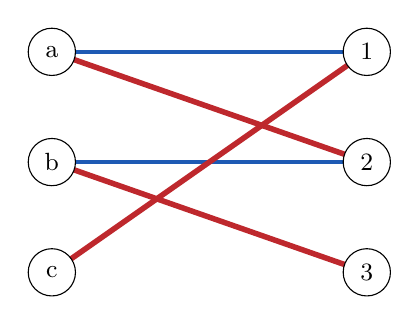
\begin{tikzpicture}[scale=1]
\coordinate (va) at (-2.000,1.400);
\coordinate (vb) at (-2.000,0.000);
\coordinate (vc) at (-2.000,-1.400);
\coordinate (v1) at (2.000,1.400);
\coordinate (v2) at (2.000,0.000);
\coordinate (v3) at (2.000,-1.400);
\draw[edge] (va)--(v1);
\draw[selected] (va)--(v2);
\draw[edge] (vb)--(v2);
\draw[selected] (vb)--(v3);
\draw[selected] (vc)--(v1);
\node[lab] at (va) {a};
\node[lab] at (vb) {b};
\node[lab] at (vc) {c};
\node[lab] at (v1) {1};
\node[lab] at (v2) {2};
\node[lab] at (v3) {3};
\end{tikzpicture}}\par\vspace{.25cm}Jeremy Quastel\end{center}\end{frame}
\begin{frame}[plain]\large \begin{center}{\Huge\bfseries Today\textquotesingle s lecture}\par\vspace{.5cm}\end{center}\begin{columns}[c,onlytextwidth]\begin{column}{.48\textwidth}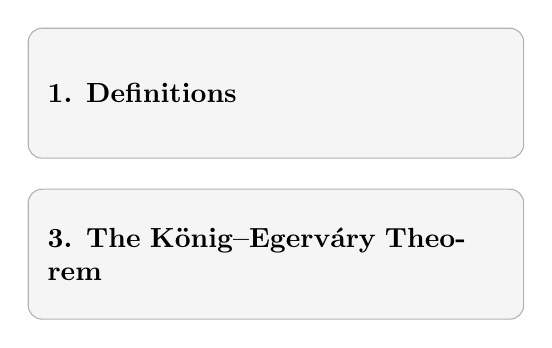
\begin{tikzpicture}\node[topic](a){\textbf{1. Definitions}};\node[topic,below=.38cm of a]{\textbf{3. The K\"onig--Egerv\'ary Theorem}};\end{tikzpicture}\end{column}\begin{column}{.48\textwidth}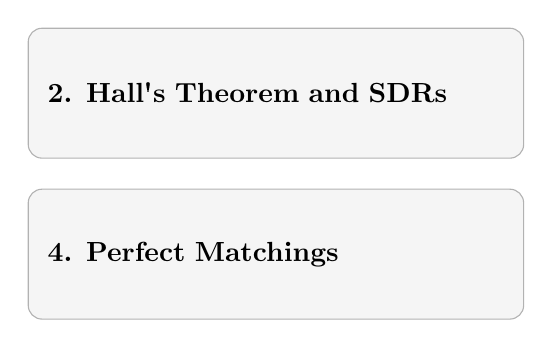
\begin{tikzpicture}\node[topic](a){\textbf{2. Hall\textquotesingle s Theorem and SDRs}};\node[topic,below=.38cm of a]{\textbf{4. Perfect Matchings}};\end{tikzpicture}\end{column}\end{columns}\end{frame}
\begin{frame}{The matching problem}
\large
\Question{A collection of jobs must be assigned to workers. Each worker can do certain jobs. When can every job be assigned to a different qualified worker?}
\gap Represent jobs and workers by the two parts of a bipartite graph. An edge records an allowed assignment.
\end{frame}
\begin{frame}{Matchings}
\large
\Def{Matching}{A \textbf{matching} in a graph is a set of edges no two of which have a common endpoint.}
\gap A vertex incident with an edge of a matching $M$ is \textbf{saturated} by $M$. Otherwise it is \textbf{unsaturated}.
\end{frame}
\begin{frame}{An example}
\large
\begin{center}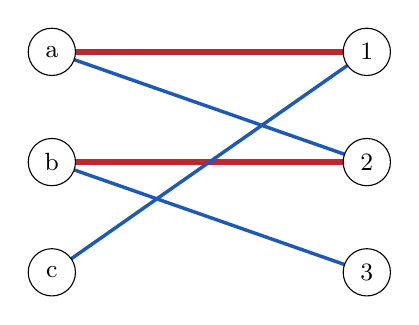
\begin{tikzpicture}[scale=1]
\coordinate (va) at (-2.000,1.400);
\coordinate (vb) at (-2.000,0.000);
\coordinate (vc) at (-2.000,-1.400);
\coordinate (v1) at (2.000,1.400);
\coordinate (v2) at (2.000,0.000);
\coordinate (v3) at (2.000,-1.400);
\draw[selected] (va)--(v1);
\draw[edge] (va)--(v2);
\draw[selected] (vb)--(v2);
\draw[edge] (vb)--(v3);
\draw[edge] (vc)--(v1);
\node[lab] at (va) {a};
\node[lab] at (vb) {b};
\node[lab] at (vc) {c};
\node[lab] at (v1) {1};
\node[lab] at (v2) {2};
\node[lab] at (v3) {3};
\end{tikzpicture}\end{center}
\begin{center}The red edges form a matching of size $2$.\end{center}
\end{frame}
\begin{frame}{Maximal and maximum matchings}
\large
\Def{Two different conditions}{A matching is \textbf{maximal} if no edge can be added to it. It is \textbf{maximum} if no matching has more edges.}
\gap In the path $v_1v_2v_3v_4$, the matching $\{v_2v_3\}$ is maximal. The matching $\{v_1v_2,v_3v_4\}$ is maximum.
\end{frame}
\begin{frame}{Perfect matchings}
\large
\Def{Perfect matching}{A matching that saturates every vertex is a \textbf{perfect matching}.}
\gap A perfect matching in a graph of order $n$ has $n/2$ edges. Thus $n$ must be even.
\gap Even order alone is not sufficient: the star $K_{1,3}$ has no perfect matching.
\end{frame}
\begin{frame}{Alternating and augmenting paths}
\large
\Def{Alternating path}{Relative to a matching $M$, an alternating path has edges alternately outside and inside $M$.}
\Def{Augmenting path}{An alternating path whose two endpoints are unsaturated is an \textbf{$M$-augmenting path}. Its first and last edges are outside $M$.}
\end{frame}
\begin{frame}{Finding an augmenting path}
\large
\begin{center}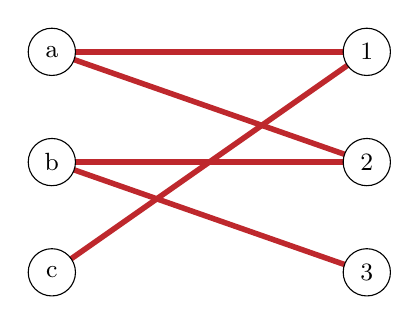
\begin{tikzpicture}[scale=1]
\coordinate (va) at (-2.000,1.400);
\coordinate (vb) at (-2.000,0.000);
\coordinate (vc) at (-2.000,-1.400);
\coordinate (v1) at (2.000,1.400);
\coordinate (v2) at (2.000,0.000);
\coordinate (v3) at (2.000,-1.400);
\draw[selected] (va)--(v1);
\draw[selected] (va)--(v2);
\draw[selected] (vb)--(v2);
\draw[selected] (vb)--(v3);
\draw[selected] (vc)--(v1);
\node[lab] at (va) {a};
\node[lab] at (vb) {b};
\node[lab] at (vc) {c};
\node[lab] at (v1) {1};
\node[lab] at (v2) {2};
\node[lab] at (v3) {3};
\end{tikzpicture}\end{center}
\begin{center}$c,1,a,2,b,3$ alternates outside and inside $M=\{a1,b2\}$.\end{center}
\end{frame}
\begin{frame}{Flipping along the path}
\large
\begin{center}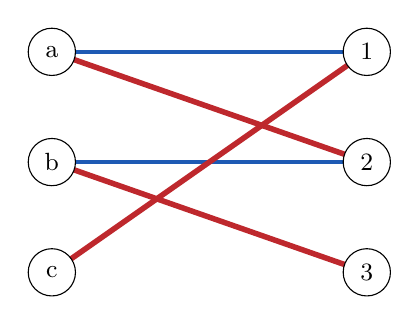
\begin{tikzpicture}[scale=1]
\coordinate (va) at (-2.000,1.400);
\coordinate (vb) at (-2.000,0.000);
\coordinate (vc) at (-2.000,-1.400);
\coordinate (v1) at (2.000,1.400);
\coordinate (v2) at (2.000,0.000);
\coordinate (v3) at (2.000,-1.400);
\draw[edge] (va)--(v1);
\draw[selected] (va)--(v2);
\draw[edge] (vb)--(v2);
\draw[selected] (vb)--(v3);
\draw[selected] (vc)--(v1);
\node[lab] at (va) {a};
\node[lab] at (vb) {b};
\node[lab] at (vc) {c};
\node[lab] at (v1) {1};
\node[lab] at (v2) {2};
\node[lab] at (v3) {3};
\end{tikzpicture}\end{center}
\begin{center}Remove $a1,b2$ and add $c1,a2,b3$. The size increases by $1$.\end{center}
\end{frame}
\begin{frame}{Berge's theorem}
\large
\Thm{Berge}{A matching $M$ is maximum if and only if there is no $M$-augmenting path.}
\Proof{An augmenting path permits a flip that increases the matching size. Therefore a maximum matching has no augmenting path.\gap For the converse, compare $M$ with a larger matching $M'$.}
\end{frame}
\begin{frame}{Berge's theorem: the converse}
\large
\Proof{Consider the graph with edge set $M\mathbin{\triangle}M'$. Every vertex has degree at most $2$, and its nontrivial components are alternating paths or even alternating cycles.\gap Each cycle has the same number of edges from the two matchings. Since $|M'|>|M|$, some path has more edges from $M'$ than from $M$.\gap That path begins and ends with edges of $M'$, and both endpoints are unsaturated by $M$. It is an $M$-augmenting path.}
\end{frame}
\begin{frame}{Neighbors of a set}
\large
\Def{Neighborhood}{For a bipartite graph with parts $X,Y$ and a set $S\subseteq X$, let
\[N(S)=\{y\in Y:xy\in E(G)\text{ for some }x\in S\}.\]}
\gap To saturate $S$, its vertices need $|S|$ distinct partners in $N(S)$.
\end{frame}
\begin{frame}{An obstruction}
\large
\begin{center}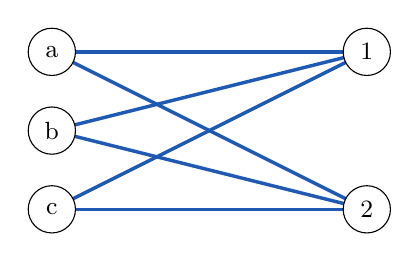
\begin{tikzpicture}[scale=1]
\coordinate (va) at (-2.000,1.000);
\coordinate (vb) at (-2.000,0.000);
\coordinate (vc) at (-2.000,-1.000);
\coordinate (v1) at (2.000,1.000);
\coordinate (v2) at (2.000,-1.000);
\draw[edge] (va)--(v1);
\draw[edge] (va)--(v2);
\draw[edge] (vb)--(v1);
\draw[edge] (vb)--(v2);
\draw[edge] (vc)--(v1);
\draw[edge] (vc)--(v2);
\node[lab] at (va) {a};
\node[lab] at (vb) {b};
\node[lab] at (vc) {c};
\node[lab] at (v1) {1};
\node[lab] at (v2) {2};
\end{tikzpicture}\end{center}
\begin{center}For $S=\{a,b,c\}$, we have $|N(S)|=2<3=|S|$.\end{center}
\end{frame}
\begin{frame}{Hall's marriage theorem}
\large
\Thm{Hall}{A bipartite graph with parts $X,Y$ has a matching saturating $X$ if and only if
\[|N(S)|\geq |S|\qquad\text{for every }S\subseteq X.\]}
\gap This condition must hold for every subset, not just for $X$ itself or for individual vertices.
\end{frame}
\begin{frame}{Hall's theorem: necessity}
\large
\Proof{Suppose a matching saturates $X$. For any $S\subseteq X$, the matching pairs the vertices of $S$ with distinct vertices of $N(S)$.\gap Consequently $|N(S)|\geq |S|$.}
\end{frame}
\begin{frame}{Hall's theorem: alternating reachability}
\large
\Proof{Assume Hall's condition, and take a maximum matching $M$. Suppose $x_0\in X$ is unsaturated.\gap Starting at $x_0$, follow edges outside $M$ from $X$ to $Y$, and matching edges from $Y$ to $X$. Let $S\subseteq X$ and $T\subseteq Y$ be the vertices reached.\gap No vertex of $T$ is unsaturated: otherwise the search gives an augmenting path, contradicting Berge's theorem.}
\end{frame}
\begin{frame}{Hall's theorem: the contradiction}
\large
\Proof{Every vertex of $T$ has its matching partner in $S$. Every vertex of $S\setminus\{x_0\}$ is reached through its matching edge and has its partner in $T$. Hence
\[|S|=|T|+1.\]
Every neighbor of $S$ lies in $T$: nonmatching edges are searched, and a matching neighbor is already reached. Also $T\subseteq N(S)$. Thus
\[|N(S)|=|T|=|S|-1,\]
contradicting Hall's condition.}
\end{frame}
\begin{frame}{Systems of distinct representatives}
\large
\Def{SDR}{Given sets $A_1,\ldots,A_n$, a \textbf{system of distinct representatives} is a choice $a_i\in A_i$ such that the chosen elements are all distinct.}
\gap Make a bipartite graph with one vertex for each set and one for each possible element. Join a set to its elements.
\end{frame}
\begin{frame}{Hall's theorem for sets}
\large
\Thm{SDR form}{The sets $A_1,\ldots,A_n$ have an SDR if and only if, for every $I\subseteq\{1,\ldots,n\}$,
\[\left|\bigcup_{i\in I}A_i\right|\geq |I|.\]}
\Example{$A_1=\{1,2\}$, $A_2=\{2,3\}$, $A_3=\{1\}$ have the SDR $(2,3,1)$.}
\end{frame}
\begin{frame}{A common mistake}
\large
\Question{If the union of $n$ nonempty sets has at least $n$ elements, must the sets have an SDR?}
\gap No. Take $A_1=A_2=\{1\}$ and $A_3=\{2,3,4\}$.
\gap The entire union is large enough, but the first two sets together have only one possible representative.
\end{frame}
\begin{frame}{Regular bipartite graphs}
\large
\Thm{Corollary}{Every $r$-regular bipartite graph with $r\geq1$ has a perfect matching.}
\Proof{Let the parts be $X,Y$. Counting edges gives $r|X|=r|Y|$, so $|X|=|Y|$. For $S\subseteq X$, all $r|S|$ edges at $S$ end in $N(S)$, which can receive at most $r|N(S)|$ edges. Thus $|S|\leq|N(S)|$. Hall gives a matching saturating $X$ and therefore also $Y$.}
\end{frame}
\begin{frame}{Decomposing a regular bipartite graph}
\large
\Thm{Corollary}{The edges of an $r$-regular bipartite graph can be partitioned into $r$ perfect matchings.}
\Proof{Remove a perfect matching. The remaining graph is $(r-1)$-regular and bipartite. Repeat, stopping when no edges remain.}
\gap Equivalently, its edges can be properly colored with $r$ colors.
\end{frame}
\begin{frame}{Vertex covers}
\large
\Def{Vertex cover}{A \textbf{vertex cover} is a set of vertices meeting every edge. Let $\tau(G)$ be its minimum size, and let $\nu(G)$ be the maximum matching size.}
\gap Every cover must meet every edge of a matching, using a different vertex for each edge. Therefore
\[\nu(G)\leq\tau(G).\]
\end{frame}
\begin{frame}{The K\"onig--Egerv\'ary theorem}
\large
\Thm{K\"onig--Egerv\'ary}{For every bipartite graph $G$,
\[\nu(G)=\tau(G).\]}
\gap The bipartite hypothesis matters. In $K_3$, a maximum matching has size $1$, while a minimum vertex cover has size $2$.
\end{frame}
\begin{frame}{Constructing a minimum cover}
\large
\Proof{Let $M$ be a maximum matching in a bipartite graph with parts $X,Y$. Start alternating searches at all unsaturated vertices in $X$. Let $Z$ be the set of vertices reached.\gap Define
\[C=(X\setminus Z)\cup(Y\cap Z).\]
We will show that $C$ covers every edge and contains exactly one endpoint of every edge in $M$.}
\end{frame}
\begin{frame}{Why the constructed set is a cover}
\large
\Proof{Suppose an edge $xy$ is not covered. Then $x\in X\cap Z$ and $y\in Y\setminus Z$.\gap If $xy\notin M$, the search reaches $y$ from $x$, a contradiction. If $xy\in M$, a reached matched vertex $x$ is reached through this matching edge, so $y$ is reached again.\gap Thus no edge is left uncovered.}
\end{frame}
\begin{frame}{Why the cover has size $|M|$}
\large
\Proof{No reached vertex in $Y$ is unsaturated, since it would finish an augmenting path. Every unsaturated vertex in $X$ is a search starting point, so it is excluded from $C$.\gap For a matching edge $xy$, its endpoints are either both reached or both unreached. In the first case only $y$ belongs to $C$; in the second only $x$ does.\gap Therefore $|C|=|M|$, proving $\tau(G)\leq\nu(G)$ and hence equality.}
\end{frame}
\begin{frame}{The matrix interpretation}
\large
\Thm{Independent entries}{In a $0$--$1$ matrix, the largest number of $1$'s with no two in the same row or column equals the smallest number of rows and columns covering all the $1$'s.}
\gap Use a bipartite graph whose parts are the rows and columns. An entry equal to $1$ gives an edge.
\gap Interchanging $0$ and $1$ gives the corresponding statement about independent zeros.
\end{frame}
\begin{frame}{Matchings as flows}
\large
\normalsize
Add a source $s$ and sink $t$ to a bipartite graph with parts $X,Y$.
\begin{itemize}
\item Direct edges $s\to x$, $x\to y$, and $y\to t$.
\item Give each edge capacity $1$.
\item An integral flow of value $k$ specifies a matching of size $k$.
\end{itemize}
\Thm{Max-flow min-cut}{The maximum flow value equals the minimum cut capacity. With integer capacities, there is an integral maximum flow.}
This gives another route to bipartite matching algorithms and theorems.
\end{frame}
\begin{frame}{Perfect matchings in general graphs}
\large
\Question{What replaces Hall's condition when the graph is not bipartite?}
\gap If $S$ is deleted, an odd component of $G-S$ cannot be matched entirely within itself. It needs an edge to a vertex of $S$.
\gap Different odd components need different vertices of $S$.
\end{frame}
\begin{frame}{Tutte's theorem}
\large
\Def{Odd components}{Write $o(H)$ for the number of connected components of $H$ having odd order.}
\Thm{Tutte}{A graph $G$ has a perfect matching if and only if
\[o(G-S)\leq |S|\qquad\text{for every }S\subseteq V(G).\]}
\end{frame}
\begin{frame}{Tutte's theorem: necessity}
\large
\Proof{Let $M$ be a perfect matching. Each odd component of $G-S$ has a vertex whose matching partner lies in $S$. Otherwise all its vertices would be paired internally, which is impossible for an odd number of vertices.\gap Matching edges from distinct odd components use distinct vertices of $S$. Thus $o(G-S)\leq|S|$.}
\end{frame}
\begin{frame}{An obstruction detected by Tutte}
\large
\Example{Take three triangles and a new vertex $v$, joined to one vertex of each triangle.}
\gap The graph has $10$ vertices. Deleting $S=\{v\}$ leaves three odd components:
\[o(G-S)=3>1=|S|.\]
\gap Hence the graph has no perfect matching, despite having even order.
\end{frame}
\begin{frame}{Tutte's theorem: sufficiency setup}
\large
\Proof{Use strong induction on the even order of $G$. The empty graph is the base case. The condition at $S=\varnothing$ implies that every component of $G$ has even order.\gap Since $|V(G)|$ is even,
\[o(G-S)\equiv |S|\pmod2.\]
Call $S$ \emph{tight} if $o(G-S)=|S|$. We distinguish whether there is a nonempty tight set.}
\end{frame}
\begin{frame}{Tutte's theorem: no nonempty tight set}
\large
\Proof{If no nonempty set is tight, parity gives
\[o(G-S)\leq |S|-2\quad(S\ne\varnothing).\]
Choose an edge $uv$; one exists because a nonempty graph satisfying the condition has no odd isolated component. Let $H=G-u-v$. For every $T\subseteq V(H)$,
\[o(H-T)=o(G-(T\cup\{u,v\}))\leq |T|.\]
By induction $H$ has a perfect matching. Adding $uv$ completes a perfect matching of $G$.}
\end{frame}
\begin{frame}{Tutte's theorem: a largest tight set}
\large
\Proof{Otherwise choose a nonempty tight set $S$ of largest possible size. There are exactly $|S|$ odd components of $G-S$.\gap There are no even components: if $C$ were even and $v\in V(C)$, then $C-v$ would have at least one odd component. Thus
\[o(G-(S\cup\{v\}))\geq |S|+1.\]
Tutte's condition forces equality, contradicting the maximal size of $S$.}
\end{frame}
\begin{frame}{Tutte's theorem: each component is factor-critical}
\large
\Proof{Let $C$ be an odd component of $G-S$ and fix $v\in V(C)$. For $T\subseteq V(C)\setminus\{v\}$, the larger set $U=S\cup\{v\}\cup T$ is not tight. Parity gives
\[o(G-U)\leq |U|-2=|S|+|T|-1.\]
The other $|S|-1$ odd components are unchanged, so
\[o(C-v-T)\leq |T|.\]
Induction gives a perfect matching in $C-v$. This holds for every $v\in V(C)$.}
\end{frame}
\begin{frame}{Tutte's theorem: use Hall's theorem}
\large
\Proof{Form a bipartite graph between $S$ and the odd components of $G-S$, joining $s$ to a component when $s$ has a neighbor there.\gap For $A\subseteq S$, deleting $S\setminus A$ leaves at least $|S|-|N(A)|$ odd components: those with no neighbor in $A$. Hence
\[|S|-|N(A)|\leq |S|-|A|.\]
Thus $|N(A)|\geq|A|$. Hall pairs every vertex of $S$ with a different component.}
\end{frame}
\begin{frame}{Tutte's theorem: finish the matching}
\large
\Proof{For each $s\in S$, choose an edge $sv$ into its paired component $C$. Match the remaining vertices of $C$ using a perfect matching of $C-v$.\gap There are exactly $|S|$ components, so each is used once. These edges and internal matchings are disjoint and saturate every vertex of $G$.}
\end{frame}
\begin{frame}{A useful sufficient condition}
\large
\Thm{Corollary of Dirac's theorem}{A simple graph of order $2n$ with minimum degree at least $n$ has a perfect matching.}
\Proof{For $n\geq2$, Dirac's theorem gives a Hamilton cycle. Its alternate edges form a perfect matching. For $n=1$, the degree condition gives the single required edge.}
\end{frame}
\begin{frame}{Practice}
\large
\Question{A bipartite graph has parts $X,Y$ of equal size. Every vertex of $X$ has degree at least $r$, and every vertex of $Y$ has degree at most $r$, where $r>0$. Prove that it has a perfect matching.}
\gap Which side of the edge count gives an upper bound? Which gives a lower bound?
\end{frame}
\begin{frame}{Practice: solution}
\large
\Proof{For $S\subseteq X$, at least $r|S|$ edges leave $S$. All end in $N(S)$, whose vertices receive at most $r|N(S)|$ edges in total. Thus
\[r|S|\leq r|N(S)|.\]
Hall's condition follows. The matching saturates $X$, and since $|X|=|Y|$, it is perfect.}
\end{frame}
\begin{frame}{Summary}
\large
\begin{itemize}
\item Augmenting paths characterize maximum matchings.
\item Hall's condition characterizes matchings saturating one part of a bipartite graph.
\item In bipartite graphs, maximum matching size equals minimum vertex cover size.
\item Tutte's odd-component condition characterizes perfect matchings in general graphs.
\end{itemize}
\end{frame}
\begin{frame}{Next time: Ramsey Theory}\begin{center}{\Huge Ramsey Theory}\end{center}\end{frame}
\end{document}